\documentclass[11pt]{article}

\usepackage{graphicx}
\usepackage{subcaption}
\usepackage{hyperref}

\usepackage[export]{adjustbox}

\usepackage[backend=bibtex]{biblatex}

\bibliography{references}

\title{Report for 194.077 Applied Deep Learning\\\vspace{15pt}CapsVoxGAN}
\author{Franz Papst}

\begin{document}

\maketitle

\section{Introduction}

My project aimed to be a three-dimensional generative adversarial network (GAN) \cite{goodfellow2014} for generating voxel models, using a three-dimensional capsule network \cite{sabour2017}.

CNNs are quite good when it comes to detecting features, but they do not take the part-to-whole-relation into account. If all features are present, but their relationship to each other is odd, a CNN would still recognise it. Figure \ref{fig:example} illustrates this: figure \ref{fig:straight} shows a simple house with normal proportions, figure \ref{fig:askew} shows how a house with skewed proportions, more resembling an abstract painting. A CNN would recognise both as house, since all the features (roof, windows and door) are there. A capsule network would take the relation of the parts to each other in account and most likely not recognise it as a house.

\begin{figure}
	\centering
	\begin{adjustbox}{minipage=\linewidth,scale=0.8}	
	\begin{subfigure}[b]{0.3\textwidth}
		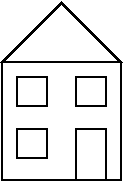
\includegraphics[width=\textwidth]{straight}
	\caption{Regular house.}
	\label{fig:straight}
	\end{subfigure}
	~
	\begin{subfigure}[b]{0.4\textwidth}
		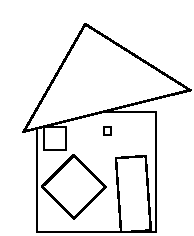
\includegraphics[width=\textwidth]{askew}
		\caption{Skewed house.}
		\label{fig:askew}
	\end{subfigure}
	\caption{Example of odd part-to-whole relation.}
	\label{fig:example}
	\end{adjustbox}
\end{figure}


\section{Fundamental Questions}

\subsection{What is the problem I tried to solve?}
I tried two tackle two different problems:
\begin{enumerate}
	\item Using a capsule network for three-dimensional model classification
	\item Generating voxel models using a GAN
\end{enumerate}

Despite the attention deep learning got in recent years, three-dimensional machine learning is still rather in its infancy. The reason for that lies in the highly increased complexity of adding one more dimension.

\subsection{Why is it a problem?}
\begin{enumerate}
	\item Magnetic resonance (MR) scans of brains are often represented in voxels \cite{chen2018b, moeskops2016}. Developing deep learning methods, which work well on this kind of data would be highly beneficial, e.g. by giving researches tools to better analyse the large scaled data-sets produced by MR, or for the automatic detection of regions of interest by physicians.
	\item While classification based on voxels can be used for very serious use-case, the ones for model generation are more light-hearted. Generating 3D models can be used in the entertainment sector for computer games or films. It would greatly cut the production costs for large and smaller studios as well as allow for new experiences, e.g. games which get generated on the fly based on the user's preferences, making it a unique experience for each player.
\end{enumerate}

\subsection{What is your solution?}
My intended solution was to build a GAN which uses a 3D capsule network as discriminator. In my actual solution, I did not use capsule networks, since I wasn't able to get them to work in 3D.

\subsection{Why is it a solution?}
Even though, the capsule network is not working as intended, the GAN is and it is able to produce voxel models as shown in figure \ref{fig:voxel_example}.

\begin{figure}
	\centering
	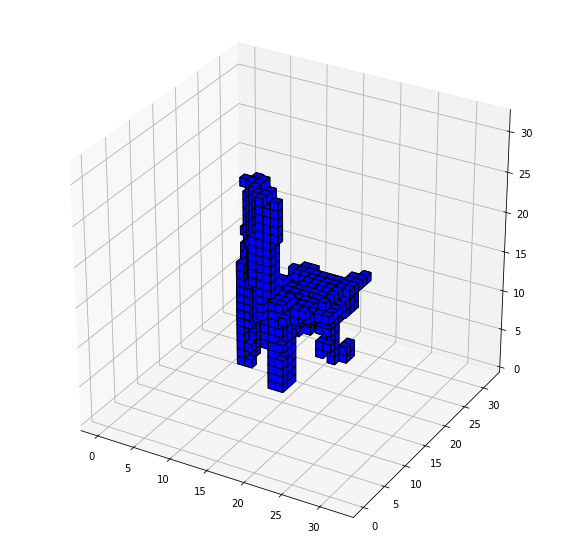
\includegraphics[width=0.7\linewidth]{../plots/epoch0490}
	\caption{Voxel model generated by the GAN after 490 training epochs.}
	\label{fig:voxel_example}
\end{figure}


\section{Main Take-Aways}
\label{sec:take-away}
Unsurprisingly the main take-away is that 3D machine learning is hard. Luckily there are datasets 3D datasets available \cite{wu2015}, but training a GAN for 3D data is still very challenging, even when having access to a GPU-cluster. In order to keep the training time reasonable, I had to limit the training data to four classes: wardrobe, bed, chair, laptop and let the training only run for 500 epochs, which took around 50 hours on a NVIDIA Tesla K20Xm with 6GB VRAM.

The results I got are reasonably good\footnote{Go to \url{https://github.com/CPUFronz/CapsVoxGAN\#results} for more examples}, but still far away from what GANs can achieve for image data. The generated models loosely resemble the training data, but when looking at them it soon becomes evident, that some voxels are missing or misplaced. This is very common when 3D models are generated by machine learning systems \cite{zhao2019b, wu2016}.

Another take-away is that reproducibility is very important. Out of my frustration with (usually) having to spend at least one day to get code found on GitHub to run (and because I was working on two different machines), I decided to use a Conda environment and make it as easy as possible for anyone who is interested, to download and run my code. It is not that much more effort and it makes things so much easier, not only for other people, but also for myself.

Related to the previous paragraph: Conda is a great tool to make development environments portable, but it is not suited for deployment (to be fair, I don't think that this was the intention behind it). I tried to create an AppImage\footnote{\url{https://appimage.org/}} out of my Conda environment, with a tool that was created for doing so\footnote{\url{https://github.com/linuxdeploy/linuxdeploy-plugin-conda}}, but it didn't really work. Afterwards I tried to put my Conda environment inside a Docker container\footnote{There are official Docker images for Miniconda: \url{https://hub.docker.com/r/continuumio/miniconda}}, but that didn't work either. In the end just using the official Docker image for PyTorch\footnote{\url{https://hub.docker.com/r/pytorch/pytorch}} and adding all the other needed packages worked best.

Speaking of deployment: deploying took actually much more time than expected. The main reason was, that creating a desktop application with a simple GUI and pack it into a AppImage, didn't work out as expected. Therefore, I had to change to a Flask\footnote{\url{https://palletsprojects.com/p/flask/}} based web app. The programming was rather easy, but turning it into a proper Docker file took some time.

In general, I have to say that I chose this project, because it is something I probably would not touch in my regular work\footnote{I mostly work with time-series data.}, but something I am interested in and want to learn more about. And indeed, I did learn a lot: from capsule networks, to 3D machine learning and deployment. It was also the first project I carried out from start to finish in PyTorch\footnote{In the past, I only used TensorFlow.}

\subsection{What would I do different, if I did the same project again?}
Start with a simple 2D capsule network for image classification or object detection and then going for something in 3D. Right from the beginning, I knew that this project is anything but easy, but 3D machine learning is hard and capsule networks are hard, so combining them is double hard. Unlike CNNs capsule networks are not shipped in popular deep learning frameworks, let alone 3D capsule networks.
%TODO 3D MNIST

Capsule networks use reconstruction as regularisation method in order to encode the instantiation parameters for a given input. This reconstruction is also generating a variation of the input, which is preserving a lot of the details, while smoothing out noise \cite{sabour2017}. For example, when trained on the MNIST data set, a capsule network reconstructs the digit it currently receives as input. This feature can be seen as an implicit generator and it should be possible to tap into it and use it for generation. It would significantly reduce the training time, since the generation would no longer be a minimax game between generator and discriminator. But since it is not trained on noise as input, it would be limited in variation. That would be something interesting to look into, but it is also out of scope for this course.


\section{Timetable}

\begin{tabular}{|c|c|c|}
	\hline 
	\textbf{Task} & \textbf{Planned Hours}  &  \textbf{Actual Hours} \\ 
	\hline 
	 Getting familiar with data / used libraries	& 10 & 10 \\ 
	\hline 
	Reading of related publications & 10 &  15 \\ 
	\hline 
	Coding of solution & 25 & 50 \\ 
	\hline 
	Deploying & - & 30 \\ 
	\hline 
	Writing report / creating presentation & 10 & 10 \\ 
	\hline 
\end{tabular}
\\

As seen in table above, I did work much more hours than originally anticipated. The reason for that is that coding needed more time than expected and deploying, which I didn't anticipate, turned out to be very time-consuming. I stated the reasons why in section \ref{sec:take-away}.

\printbibliography

\end{document}
